
The PCC luminosity determination requires corrections for ``afterglow'' effects, noise induced in bunch crossings following colliding bunch crossings.
Two corrections have been previously developed: Type-1 refers to a spill over into the bunch crossing immediately following an active bunch crossing due to charge residuals in the pixel sensors, the second Type-2 refers to exponentially decaying noise created by activated material.
The models for both corrections are normalized using data from empty bunch crossings recorded with \random\ triggers.
The corrections are stored in the CMS Conditions Database during the Prompt Calibration Loop (PCL).
The PCC values obtained from the \zerobias\ trigger data are then corrected in an offline analysis.
Similar afterglow corrections are obtained for HFOC.

The afterglow corrections are normally calculated for an integrated range of lumi sections to improve the statistical precision, for PCC every 50 LS while for HFOC every 20. In this study the PCC corrections were determined privately every 10 LS to capture variations during $\mu$-scans.
Example corrections (Type-1 and Type-2 combined) are showin in Figure~\ref{fig:afterglow}.
For fill 6847 the corrections have values of 1.0 due to the single bunch pattern.

\begin{figure}[t]
  \begin{center}
    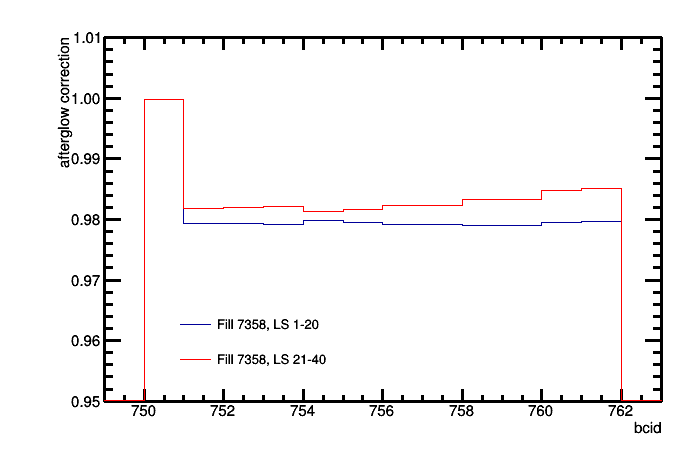
\includegraphics[width=0.47\linewidth]{plots/HFAfterglowCorr.png}
    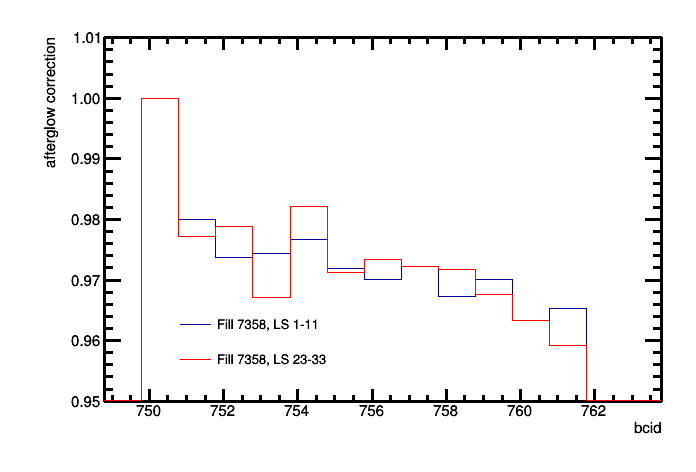
\includegraphics[width=0.47\linewidth]{plots/PCCAfterglowCorr.png}
    \caption{
      Afterglow corrections for HFOC (left) and PCC (right) as a function of bcid for one bunch train in fill 7358.
      The different curves show the difference between low and high pileup lumisections.
    \label{fig:afterglow}
    }
  \end{center}
\end{figure}

